\documentclass[lang=cn,11pt,chinesefont=nofont]{elegantbook}

% 字体配置:
% macOS:   fontset=macnew  或 fontset=mac
% Windows: fontset=windowsnew 或 fontset=windows
% Linux:   fontset=ubuntu 或 fontset=fandol
% 如果注释掉 fontset,ctex 会尝试自动检测系统字体
%\usepackage[UTF8,scheme=plain,fontset=macnew]{ctex}
\usepackage[UTF8,scheme=plain]{ctex}



\title{Math 525}

\begin{document}
\frontmatter
\tableofcontents
\mainmatter

% 包含各个章节
% \chapter{basic combinatorics}
\begin{definition}{permutations}
一个 permutation 就是对一组 objects 的一个 \textbf{rearrangement} (这些 objects 中可以有 same 的也可以有 distinct 的).\\
    对于 $n$ 个 \textbf{distinct objects}, 一共存在 \(n! = n(n-1)(n-2)\cdots \) 个 permutations.
\end{definition}

\begin{example}
    \# distinct permutations of "STATISTICS"?\\
    这里一共有 10 个 objects. 但问题是: 其中有 3 个 \(S\), 3 个 \(T\), 2 个 \(I\) 是相同的.\\
    于是: 我们首先假设它们都是 distinct 的, 则存在 \(10!\) 个 permutations. 而, 每个 permutation 都包含了对 3 个 $S$ 的一个子 permutation. 而对 3 个 $S$ 的任意 permutation 都是相同的! 同样的道理 apply to 3 个 $T$ 和 2 个 $I$.\\
    所以这个结果是真实结果的 \(3!3!2!\) 倍.\\
    同样地, 由于
    因而, 正确结果是: \[
    \frac{10!}{3!3!2!1!1!}
    \]
\end{example}
\begin{remark}
    这个地方解释一下为什么是 $3!3!2!1!1!$ 而不是 $3!3!2!1!1!1!$
    
\end{remark}

\begin{definition}{combinations}
从 $n$ 个 objects 中选取 $k$ 个的 ways 为: \[
\binom{n}{k} = \frac{n!}{k!(n-k)!}
\]

\end{definition}

% \chapter{Probability space intro}
\section{probability space}
我们这里跳过所有 measure theory 的内容, 见 notes on measure theory.\\
\begin{definition}{prob space, prob measure, sample space, event space}
    一个 probability space 就是一个 measure space \( (\Omega, \mathcal{F}, \mathbb{P}) \), 其中 $\mathbb{P}(\emptyset) =0, \mathbb{P}(\Omega) = 1$.\\
    对于这样的 measure $\mathbb{P}$, 我们称之为 \textbf{probability measure (概率测度, 即概率)}.\\
    而这里的 \(\Omega\) 我们称之为 \textbf{sample space (样本空间)}; 这里的 $\sigma$-algebra $\mathcal{F}$, 我们称之为 \textbf{event space (事件空间)}. \\
    任意的 $A \subset \Omega$ 都是一个 \textbf{event}, 但是概率论中只考虑 $A\in\mathcal{F}$, 即 measurable event. 为简化, event 这个单词就指 measurable event.
\end{definition}
\begin{remark}
    回顾一下 measure space 的定义:
    \begin{itemize}
        \item 一个 set $\Omega$ 的一个 $\sigma$-algebra 就是一个包含空集的子集簇, 其 \textbf{closed under countable unions and complements}. (如果只 closed under finite unions, 则只称为一个 algebra.)
        \item 一个 Borel algebra 是一个定义在 topological space 上的 $\sigma$-algebra, 由 all open sets 生成. (因而: closed under countable unions and complements.) $\mathbb{R}$ 的 Borel algebra 可以由 all open intervals 生成.
        \item 一个 measure on a measurable space $(\Omega, \mathcal{F})$ 就是一个从 $\mathcal{F} \to \mathbb{R}$ 的函数, 满足 \textbf{countable additivity}.
        \item measure 的性质: \textbf{(1)non-negativity, (2) monotonicity, (3) countable subadditivity, (4) inclusion-exclusion principle (上节已讲), (5) continuity from below and above.} 第 (5) 条具体即:
        For measurable sets $A_1 \subseteq A_2 \subseteq \cdots \subseteq A_n \subseteq \cdots$, then $\lim_{n \to \infty} \mathbb{P}(A_n) = \mathbb{P}(\bigcup_{n=1}^{\infty} A_n)$.\\
        For measurable sets $A_1 \supseteq A_2 \supseteq \cdots \supseteq A_n \supseteq \cdots$, then $\lim_{n \to \infty} \mathbb{P}(A_n) = \mathbb{P}(\bigcap_{n=1}^{\infty} A_n)$.
    \end{itemize}
\end{remark}
\begin{remark}
    对于 discrete 的 prob space 而言, 通常选取 $\mathcal{F} = 2^{\Omega}$, 即 $\Omega$ 的任意子集都是一个 event.
\end{remark}
\begin{remark}
    概率空间的现实意义是: 一次 experiment 的所有可能的结果的集合, 以及每个结果的概率.
    \begin{align*}
        \Omega &= \{\omega \mid \omega \text{ 是一次 experiment 的可能的结果}\}\\
        \mathbb{P}(\omega) &= \text{ 结果 $\omega$ 的可能性}
    \end{align*}
\end{remark}

\begin{example}
    (dice roll) 
    如果我们掷一个 6 面的骰子, 那么样本空间 $\Omega=\{1,2,3,4,5,6\}$. 一个可能的事件是 $A=\{1,2\}$. 如果假设骰子是公平的 (所有结果都是等可能的), 那么事件 $A$ 的概率是
    \[
    \mathbb{P}(A)=\frac{\text { Number of favorable outcomes }}{\text { Total number of outcomes }}=\frac{|A|}{|\Omega|}=\frac{2}{6} 
    \]
    % 如果我们定义一个随机变量 $X$ 表示掷骰子的结果, 那么 $X$ 的样本空间是 $\mathbb{R}$, 即 $X: \Omega \rightarrow \mathbb{R}$. 
    % 那么 $X$ 的分布函数是
    % \[
    % F_X(x) = \mathbb{P}(X \leq x) = \begin{cases}
    %     0, & x < 1 \\
    %     1/6, & 1 \leq x < 2 \\
    %     2/6, & 2 \leq x < 3 \\
    % \end{cases}
    % \]
    根据我们 measure-based 的定义, 这一结果自然 follows from countable additivity of $\mathbb{P}$.
\end{example}




\begin{example}
    三个人独立地掷一个 6 面的骰子, 求第三个人掷出的点数等于前两个人的点数之和的概率.
    \begin{solution}
        样本空间 $\Omega=\{1,2,3,4,5,6\}^3$.
        event: $E = \{ \omega \in \Omega \mid \omega_3 = \omega_1 + \omega_2 \}$.\\
        这个 event 有 15 个 elements: \[
        E = \{ (1,1,2), (1,2,3), (1,3,4), \cdots, (2,1,3), (2,2,4), \cdots, (3,1,4), \cdots, (4,1,5), \cdots, (5,1,6) \}
        \]
        因此, 概率是: \[
        \mathbb{P}(A)=\frac{|A|}{|\Omega|}=\frac{15}{216}=\frac{5}{72}
        \]
    \end{solution}
\end{example}


\begin{example}
    两个人计划在 12:00 到 1:00 之间碰面. 他们各自都会在期间的某个时间点到达. 求: 他们彼此不会等待对方超过 10 分钟的概率.\\
    \begin{solution}
        Sample space $$\Omega = \{(x,y): 0\leq x \leq 60, 0\leq y \leq 60\} = [0,60] \times [0,60]$$
        我们要求概率的事件 \[
        E = \{ (x,y)\in \Omega : |x-y| \leq 10 \} 
        \]
        容易画出图像:
        \begin{center}
        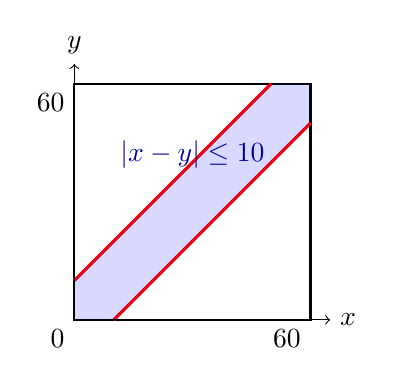
\begin{tikzpicture}[scale=0.05]
            % 绘制正方形区域
            \draw[thick] (0,0) rectangle (60,60);
            % 绘制两条界限直线: x-y=10  与 x-y=-10
            \draw[red,very thick] (10,0) -- (60,50);   % x - y = 10
            \draw[red,very thick] (0,10) -- (50,60);   % x - y = -10
            % 填充有效区域
            \fill[blue,opacity=0.15] 
                (0,10) -- (10,0) -- (60,50) -- (50,60) -- cycle;
            % 漏画了两个小的角
            \fill[blue,opacity=0.15]
                (0,0) -- (0,10) -- (10,0) -- cycle;
            \fill[blue,opacity=0.15]
                (60,60) -- (60,50) -- (50,60) -- cycle;
            % 坐标轴
            \draw[->] (0,0) -- (65,0) node[right] {$x$};
            \draw[->] (0,0) -- (0,65) node[above] {$y$};
            % 标注几个重要点
            \foreach \p/\lab in {(0,0)/0, (60,0)/60, (0,60)/60} {
                \draw \p node[below left]{\lab};
            }
            % 标签
            \node[blue!60!black] at (30,42) {$|x-y|\leq 10$};
        \end{tikzpicture}
        \end{center}
        因而概率是
        \[
        \mathbb{P}(E) = \frac{m(E)}{m(\Omega)} = \frac{3600-2500}{3600} = \frac{11}{36}
        \]
    \end{solution}
\end{example}



\section{conditional probability and independence}
\begin{definition}{conditional probability}
    对于 probability space \((\Omega, \mathcal{F}, \mathbb{P})\), 给定一个 event $B \in \mathcal{F}$, 我们定义 conditional probability of an event $A \in \mathcal{F}$ given $B$ 为:
    \[
    \mathbb{P}(A \mid B) = \frac{\mathbb{P}(A \cap B)}{\mathbb{P}(B)}
    \]
\end{definition}
\begin{proposition}{decomposing probability of intersection of events}   
    令 $\left(A_i\right)_{i \in \mathbb{N}}$ 为一个 seq of events, 对于任意 $n \in \mathbb{N}$:
    \[
    \mathbb{P}\left(A_1 \cap A_2 \cap \ldots \cap A_n\right)=\mathbb{P}\left(A_1\right) \cdot \mathbb{P}\left(A_2 \mid A_1\right) \cdot \mathbb{P}\left(A_3 \mid A_1 \cap A_2\right) \ldots \cdot \mathbb{P}\left(A_n \mid A_1 \cap \ldots \cap A_{n-1}\right)
    \]
\end{proposition}
\begin{proof}
Naturally follows from the def. 
\end{proof}


\begin{theorem}{law of total probability}
    令 $\left(A_i\right)_{i \in \mathbb{N}}$ 为一个 seq of \textbf{pairwise disjoint} events, 如果 $\sqcup_{i=1}^{\infty} A_i=\Omega$, 那么对于任意 event $E \subseteq \Omega$:
    \[
    \mathbb{P}(E)=\sum_{i=1}^{\infty} \mathbb{P}\left(A_i\right) \mathbb{P}\left(E \mid A_i\right)
    \]
\end{theorem}
\begin{proof}
    \[
    \mathbb{P}(E)=\mathbb{P}\left(E \cap \cup_{i=1}^{\infty} A_i\right)=\mathbb{P}\left(\cup_{i=1}^{\infty} E \cap A_i\right)=\sum_{i=1}^{\infty} \mathbb{P}\left(E \cap A_i\right)=\sum_{i=1}^{\infty} \mathbb{P}\left(A_i\right) \mathbb{P}\left(E \mid A_i\right)
    \]
\end{proof}
\begin{remark}
    \(P(A_i)P(E\mid A_i)\) 就等于 \(P(E \cap A_i)\), 也就是在 \(A_i\) 这个区域上, \(E\) 的 measure. 因而 disjoint union 之下就是 \(E\) 的完整 measure.
\end{remark}

\begin{theorem}{Bayes theorem}
    If $A, B \subseteq \Omega$ such that $\mathbb{P}(B) \neq 0$, then
    \[
    \mathbb{P}(A \mid B)=\frac{\mathbb{P}(A) \cdot \mathbb{P}(B \mid A)}{\mathbb{P}(B)}
    \]
\end{theorem}
\begin{remark}
    这其实是一个非常直接的结果, 因为 \(P(A) \dot P(B \mid A) = P(A \cap B)\). \\
    但是它的意义在于, 如果我们知道两个事件的概率和其中一个对另一个的条件概率, 我们就也得到了反过来的条件概率.
\end{remark}



\begin{example}{(Medical testing)}

在一个群体中, 随机选取一个人患有某种罕见疾病的概率是 0.001. 该疾病有一个诊断测试, 其性质如下: 给定个体患病, 测试呈阳性的概率 (真正阳性率) 是 0.99. 给定个体健康, 测试呈阳性的概率 (假阳性率) 是 0.02. 从群体中随机选取的一个人测试呈阳性. 该个体实际上患有该疾病的概率是多少?
于是
\begin{solution}
由 law of total probability, 我们有
\[
 \mathbb{P}(\text {positive})= \mathbb{P}(\text{positive} \mid \text{sick}) \mathbb{P}(\text{sick}) + \mathbb{P}(\text{positive} \mid \text{healthy}) \mathbb{P}(\text{healthy}) = 0.99 \cdot 0.001 + 0.02 \cdot 0.999 = 0.02097
\]
于是
\[
\mathbb{P}(\text {sick} \mid \text {positive})=\frac{0.99 \cdot 0.001}{0.02097} \approx 0.047
\]
\end{solution}
\end{example}

\begin{example}{(Monty Hall problem)}
假设你参加一个游戏节目, 面前有三扇门: 一扇门后面有一辆车; 其他两扇门后面是山羊. 你选择了一扇门, 比如说是 1 号门, 然后主持人 (他知道每扇门后面是什么) 打开了另一扇门, 比如说是 3 号门, 里面有一只山羊. 然后他说 "你想换成 2 号门吗?". 换门对你有利吗?
\begin{solution}
令 \(A_i\) 表示: car 在 \(i\) 号门后面; \(B\) 事件表示: 主持人打开 3 号门. 我们要求的概率是在事件 \(B\) 发生的情况下, \(A_2\) 的个概率, 即 \(\mathbb{P}(A_2 \mid B)\). 它的大小是:
\begin{align*}
\mathbb{P}(A_2 \mid B) &= \frac{\mathbb{P}(A_2) \cdot \mathbb{P}(B \mid A_2)}{\mathbb{P}(B)} \\
&= \frac{\mathbb{P}(B \mid A_2)\mathbb{P}(A_2)}{\mathbb{P}(B\mid A_1)\mathbb{P}(A_1) + \mathbb{P}(B\mid A_2)\mathbb{P}(A_2) + \mathbb{P}(B\mid A_3)\mathbb{P}(A_3)}    \\
&= \frac{1 \cdot \frac{1}{3}}{\frac{1}{2} \cdot \frac{1}{3} + 1 \cdot \frac{1}{3} + 0 \cdot \frac{1}{3}} = \frac{2}{3} > \frac{1}{3}
\end{align*}
因而, 换门是有利的.
\end{solution}
\end{example}
% \chapter*{Homework 1}



\section*{Problem 1}
Let $n \in \mathbb{N}$.
\begin{itemize}
    \item[(a)] Show that $2^n=\sum_{k=0}^n\binom{n}{k}$. Given that a set of $n$ elements has $2^n$ subsets, what is the combinatorial interpretation of this equality?
    \item[(b)] Show that $$\sum_{k \text { odd }, 0 \leq k \leq n}\binom{n}{k}=\sum_{k \text { even }, 0 \leq k \leq n}\binom{n}{k} $$
    \item[(c)] Show that $$\binom{2 n}{n}=\sum_{k=0}^n\binom{n}{k}^2 $$
\end{itemize}
Hint: You may use $\binom{n}{k}^2=\binom{n}{k}\binom{n}{n-k}$.
\begin{proof}
    \begin{itemize}
        \item[(a)] 
By the binomial theorem, we have:
\[
(1+1)^n = \sum_{k=0}^n \binom{n}{k} 1^k 1^{n-k} = \sum_{k=0}^n \binom{n}{k}
\]
The combinatorial interpretation of this equality is that:
Let $S_k$ be the collection of all subsets that have size $k$.
For collection $S_k$, its size is $\binom{n}{k}$ since it represents choosing $k$ elements from $n$ elements without regard to order.\\
Therefore the total number of subsets of $S$ is:
\[
| \mathcal{P}(S) |=\sum_{k=0}^n |S_k|  =\sum_{k=0}^n \binom{n}{k} =2^n
\]        
        \item[(b)] 
Using the binomial theorem, we have:
\[
0 = (1-1)^n = \sum_{k=0}^n \binom{n}{k} (-1)^k 1^{n-k} = \sum_{k=0}^n \binom{n}{k} (-1)^k
\]
Thus:
\begin{align}
    &\quad\quad\quad\quad \sum_{k=0}^n \binom{n}{k} (-1)^k = 0 \nonumber \\
    &\implies \sum_{0\leq k \leq n,\, k \text{ odd} } \binom{n}{k} (-1)
    + \sum_{0\leq k \leq n,\, k \text{ even} } \binom{n}{k} (1) = 0 \nonumber \\
    &\implies \sum_{0\leq k \leq n,\, k \text{ odd} } \binom{n}{k}
    = \sum_{0\leq k \leq n,\, k \text{ even} } \binom{n}{k}
\end{align}
        \item[(c)] 
We prove by combinatorial argument.\\
Let $S$ be a setwith $2n$ distinct elements. The number of ways to choose a subset $P$ containing $n$ elements is $\binom{2n}{n}$.\\
In another way: 
We can first arbitrarily divide the $2n$ distinct elements into two groups: group $A$ and group $B$, each containing $n$ elements:
\[
S = A \sqcup B
\]
And fix the two groups. \\
For any subset $P$ of the $2n$ elements with size $n$, some of them are from group $A$, and the rest of them are from group $B$. \\
Let $k$ be the number of elements of $P$ that are chosen from $A$, then the number of elements chosen from $B$ must be $n-k$.\\
Note the number of ways to choose $k$ elements from $A$ is $\binom{n}{k}$, and the number of ways to choose $n-k$ elements from $B$ is $\binom{n}{n-k}$. \\
Therefore, the total number of ways to get $P$ from $S=A \sqcup B$ with $k$ elements from $A$ is $\binom{n}{k}\binom{n}{n-k} = \binom{n}{k}^2$.\\
Thus, summing over all possible values of $k=0,1,\dots,n$, the number of ways to choose $n$ elements from $S$ i.e. the number of ways to get $P$ from $S$, is $$\sum_{k=0}^n \binom{n}{k}^2$$
Thus, we obtain $$\binom{2n}{n}=\sum_{k=0}^n \binom{n}{k}^2$$ as desired.
    \end{itemize}
\end{proof}


\section*{Problem 2}
We roll a fair die three times and record the outcomes $a, b, c \in\{1,2,3,4,5,6\}$. What is the probability that the equation $a x^2+b x+c=0$ does not have solutions in the real numbers?
\begin{solution}
    The equation $a x^2+b x+c=0$ does not have solutions in the real numbers iff the the discriminant is negative, i.e. $\Delta=b^2-4 a c<0$.\\
    Total possible equations is $6^3 = 216$. For each $b$, the total possible $(a,c)$ pairs are $36$. We can calculate the number of $(a,c)$ pairs that satisfy the condition case by case.
\begin{itemize}
\item For $b=1$: $4ac > 1$ holds for all $(a,c)$.
\item For $b=2$: $4ac > 4 \implies ac > 1$, which excludes only $(1,1)$.
\item For $b=3$: $4ac > 9 \implies ac \ge 3$ since they are integers, so excluding $(1,1),(1,2),(2,1)$ ($3$ cases).
\item For $b=4$: $4ac > 16 \implies ac \ge 5$, excluding: $(1,3),(1,4),(2,2),(3,1),(4,1)$ besides the previous case, thus $8$ cases excluded.
\item For $b=5$: $4ac > 25 \implies ac \ge 7$, excluding: $(1,5),(1,6),(2,3),(3,2),(5,1),(6,1)$ besides the previous case, thus $14$ cases excluded.
\item For $b=6$: $4ac > 36 \implies ac \ge 10$, excluding: $(2,4),(3,3),(4,2)$ besides the previous case, thus $17$ cases excluded.
\end{itemize}
Thus, the total number of triples for which the discriminant is not negative (exlcuded) is
\[
1+ 3 + 8 + 14 + 17 = 43
\]
Therefore, the desired probability is
\[
1-\mathbb{P}(\text{the equation has solutions in the real numbers}) = 1-\frac{43}{216} = \frac{173}{216}
\]
\end{solution}


\section*{Problem 3}
An ant starts at the origin $(0,0)$ on the integer lattice.
At each step it moves either one unit to the right or one unit upward, each with probability $\frac{1}{2}$. 
The ant continues moving until it reaches the point $(205,200)$.\\
What is the probability that the ant visits the point $(105,100)$ at some time during its journey?\\
Hint: Start by counting the number of paths from $(0,0)$ to $(205,200)$.
\begin{solution}
Any path from $(0,0)$ to $(205,200)$ must consist of $205$ steps to the right and $200$ steps upward, for a total of $405$ steps. 
So a path is uniquely determined by the choice of 205 steps to the right (which is equivalent to the choice of 200 steps upward).\\
Thus total number of paths from $(0,0)$ to $(205,200)$ is
\[
N = \binom{405}{205}
\]

A path passes through the point $(105,100)$ if and only if it first goes from $(0,0)$ to $(105,100)$ and then from $(105,100)$ to $(205,200)$.\\
Thus the number of such paths is the product of the number of paths from $(0,0)$ to $(105,100)$ and the number of paths from $(105,100)$ to $(205,200)$, by the fundamental counting principle.
For the same reason as deciding the number of total paths from $(0,0)$ to $(205,200)$, the number of paths from $(0,0)$ to $(105,100)$ is
\[
N_1 = \binom{205}{105}
\]
And similarly, the number of paths from $(105,100)$ to $(205,200)$ is
\[
N_2 = \binom{200}{100}
\]
Note that from a point to another point, all such paths are equally likely to be chosen. Therefore, the desired probability is
\[
\mathbb{P}(\text{path passes through $(105,100)$}) = \frac{\binom{205}{105}\binom{200}{100}}{\binom{405}{205}}
\]
\end{solution}

\section*{Problem 4}
From a lottery containing $n$ tickets numbered $1,2, \ldots, n$, a ticket is drawn, its number is recorded, and then it is returned to the lottery. This process is repeated $k \geq 3$ times. Find the probabilities of the following events:
\begin{itemize}
    \item[(a)] Ticket 1 is selected at least once.
    \item[(b)] Tickets 1, 2, and 3 are each selected at least once.
\end{itemize}
\begin{solution}
\begin{itemize}
    \item[(a)] 
 Let $E$ be the event that ticket $1$ is selected at least once.
 \begin{align*}
    \mathbb{P}(E) &= 1 - \mathbb{P}(\text{ticket $1$ is never selected in $k$ draws}) \\
    &= 1 - \left(\frac{n-1}{n}\right)^k \tag*{\text{(by independence of each draw)}}
 \end{align*}
    \item[(b)] 
Let $F$ be the event that tickets $1,2,3$ are each selected at least once. \\
For $i=1,2,3$, let
\[
A_i:=\{\text{ticket } i \text{ is never selected in the } k \text{ draws}\}
\]
Thus 
\[
P(F) = 1 - P(A_1 \cup A_2 \cup A_3)
\]
By the principle of inclusion-exclusion,
\[
P(A_1 \cup A_2 \cup A_3) = P(A_1) + P(A_2) + P(A_3) - P(A_1 \cap A_2) - P(A_1 \cap A_3) - P(A_2 \cap A_3) + P(A_1 \cap A_2 \cap A_3)
\]
Since similar to part (a), we have:\(\mathbb{P}(A_i)=\left(\frac{n-1}{n}\right)^k\), \(\mathbb{P}(A_i\cap A_j)=\left(\frac{n-2}{n}\right)^k\), \(\mathbb{P}(A_1\cap A_2\cap A_3)=\left(\frac{n-3}{n}\right)^k\), we then calculate:
\begin{align*}
\mathbb{P}(F) &= 1 - \binom{3}{1}\left(\frac{n-1}{n}\right)^k + \binom{3}{2}\left(\frac{n-2}{n}\right)^k - \binom{3}{3}\left(\frac{n-3}{n}\right)^k\\
&=1-3\left(\frac{n-1}{n}\right)^k+3\left(\frac{n-2}{n}\right)^k-\left(\frac{n-3}{n}\right)^k
\end{align*}
\end{itemize}
\end{solution}



\section*{Problem 5}
In a house, drawer $S_1$ contains 3 gold coins and 3 silver coins, 
while drawer $S_2$ contains 3 gold coins and 6 silver coins. 
A thief (in the dark) randomly opens one drawer and then randomly takes two coins from it.
\begin{itemize}
    \item[(a)] What is the probability that both coins are gold?
    \item[(b)] If it is discovered (upon his arrest) that he has stolen two gold coins, what is the probability that he opened drawer $S_1$ ?
\end{itemize}
\begin{solution}

The thief chooses a drawer uniformly at random, so for each pick, $\mathbb{P}(\text{$S_1$ is chosen}) = \mathbb{P}(\text{$S_2$ is chosen}) = \frac12$. 
Given a drawer, he draws two coins without replacement.
\begin{itemize}
\item[(a)] Using the law of total probability,
\begin{align*}
\mathbb{P}(\text{two gold}) &= \mathbb{P}(\text{two gold}\mid S_1 \text{ is chosen})\mathbb{P}(\text{drawer $S_1$}) + \mathbb{P}(\text{two gold}\mid S_2 \text{ is chosen})\mathbb{P}(\text{drawer $S_2$}) \\
&= \frac{1}{2} \cdot \frac{\binom{3}{2}}{\binom{6}{2}} + \frac{1}{2} \cdot \frac{\binom{3}{2}}{\binom{9}{2}} \\
&= \frac{1}{2} \left( \frac{3}{15} + \frac{3}{36} \right) \\
&= \frac{36 + 15}{360}\\
&= \frac{17}{120}
\end{align*}
\item[(b)] 
Let $G$ be the event that the thief stole two gold coins. By Bayes' rule,
\[
\mathbb{P}(S_1\mid G)=\frac{\mathbb{P}(G\mid S_1)\mathbb{P}(S_1)}{\mathbb{P}(G)}
\]
Since we have $\mathbb{P}(G\mid S_1)=\frac{\binom{3}{2}}{\binom{6}{2}}=\frac15$, $\mathbb{P}(S_1)=\frac12$, and $\mathbb{P}(G)=\frac{17}{120}$ from part (a), we get:
\[
\mathbb{P}(S_1\mid G)=\frac{\frac15\cdot \frac12}{\frac{17}{120}}
=\frac{12}{17}
\]
\end{itemize}
\end{solution}


\section*{Problem 6}
Let $A$ and $B$ be events of a probability space with $\mathbb{P}(A)>0$. Show that:
\begin{itemize}
    \item[(a)] $\mathbb{P}(A \cup B)>0$ and $\mathbb{P}(A \cap B \mid A \cup B) \leq \mathbb{P}(A \cap B \mid A)$.
    \item[(b)] $\mathbb{P}(B \mid B \cup A) \geq \mathbb{P}(B \mid A)$.
\end{itemize}
\begin{proof}

\begin{itemize}
\item[(a)] Since $A\subseteq A\cup B$, we have by monotonicity of probability measure:
\[
\mathbb{P}(A\cup B)\ge \mathbb{P}(A)>0
\]
Also, since $A\cap B\subseteq A$ and $\mathbb{P}(A\cup B)\ge \mathbb{P}(A)>0$, 
both conditional probabilities below are well-defined. 
Then
\begin{align*}
\mathbb{P}(A\cap B\mid A\cup B)
&=\frac{\mathbb{P}((A\cap B) \cap (A\cup B))}{\mathbb{P}(A\cup B)} \\
&= \frac{\mathbb{P}(A\cap B)}{\mathbb{P}(A\cup B)} \\
&\le \frac{\mathbb{P}(A\cap B)}{\mathbb{P}(A)}\\
&=\mathbb{P}(A\cap B\mid A)
\end{align*}
This finishes the proof.
\item[(b)] 
Let \(x:=\mathbb{P}(A\cap B)\), \(y:= \mathbb{P}(A\setminus B)\), \(z:= \mathbb{P}(B\setminus A)\).\\
so $x,y,z\ge 0$ by non-negativity of probability measure.\\
And since \[
A = (A\cap B) \sqcup (A\setminus B)
\]
Thus, we have: 
\[
\mathbb{P}(A)=\mathbb{P}(A\cap B)+\mathbb{P}(A\setminus B)=x+y
\]
By similar reason, we have:
\[
\mathbb{P}(A\cup B)=x+y+z,\quad \mathbb{P}(B)=x+z
\]
Thus we have:
\[
\mathbb{P}(B\mid A\cup B)= \frac{\mathbb{P}(B \cap (A\cup B))}{\mathbb{P}(A\cup B)} = \frac{\mathbb{P}(B)}{\mathbb{P}(A\cup B)}=\frac{x+z}{x+y+z}
\]
and 
\[
\mathbb{P}(B\mid A)=\frac{\mathbb{P}(A\cap B)}{\mathbb{P}(A)}=\frac{x}{x+y}
\]
Note the two probabilities are well-defined since $x+y= \mathbb{P}(A)>0$ (and so $x+y+z>0$).\\
Now it remains to show that:
\[
\frac{x+z}{x+y+z}\ge \frac{x}{x+y}
\]
i.e. \[
(x+z)(x+y)\ge x(x+y+z)
\]
which is equivalent to:
\[
x(x+y)+z(x+y) \geq x(x+y)+x z
\]
Eliminating common terms, this is equivalent to:
\[
zy \geq 0
\]
which is true by non-negativity of $z$ and $y$. This finishes the proof that:
\[
\mathbb{P}(B\mid A\cup B)\ge \mathbb{P}(B\mid A)
\]
\end{itemize}
\end{proof}

% \chapter{random variables}

随机变量 $X: \Omega \rightarrow \mathbb{R}$ 就是一个从样本空间 \((\Omega, \mathcal{F},P)\) 到 $\mathbb{R}$ 的 measurable function.\\

其 cdf $F_X: \mathbb{R} \rightarrow [0,1]$ 就是 $X$ 这个 real-valued measurable function 对于 $(-\infty,x]$ 的 preimage, 意义是 "随机变量的值小于等于 $x$ 的概率"  \[
F_X (x) = P( X^{-1}(-\infty,x])
\]
discrete random variable 的 pmf, 表示每个离散点 $x$ 的 $P(X^{-1}(\{x\}))$.
即 \[
p(x) := P(X^{-1}(\{x\})) = P(X=x)
\]
continuous random variable 的 pdf, 表示在某个点上概率分布的密度有多大 \[
f_X(x) :=  \frac{dF_X(x)}{dx}
\]
或者写作: \[
f_X(x) :=  \frac{dF_X(x)}{dm}
\]
是这个 $F_X$ 对于 Lebesgue measure $m$ 的 Radon-Nikodym derivative.


随机变量的 expectation 是它在这个 prob space 上的积分, 表示它的值的 prob-weighted average
\[
E (X):= \int_\Omega X  \;d P
\]
随机变量的 variance 是 $(X-E(X))^2$ 这个 induced 随机变量在这个 prob space 上的积分, 表示原随机变量值离它的值的 weighted average 的聚集程度. \[
Var(X) = \int_\Omega (X-E(X))^2   \;dP
\]










% \input{chapters/ch04-continuous-random-variables}
% \chapter{joint probability}


\begin{example}
    Suppose $X,Y$ 是 independent normal r.v., with mean 0 and 
\end{example}










\chapter*{Homework 2}
\section*{Problem 1}
Suppose that the cumulative distribution function (CDF) of a random variable $F: \mathbb{R} \rightarrow \mathbb{R}$ is strictly increasing and continuous. Let $U$ be a random variable with the uniform distribution on $(0,1)$ and define
$$
X:=F^{-1}(U) .
$$
Show that $X$ has CDF equal to $F$.
This exercise shows us how to construct a random variable with given distribution, assuming that we have a uniform random variable.
\begin{proof}
Since $F$ is strictly increasing and continuous, it has an inverse function $F^{-1}$ on its range, and $F^{-1}$ is also strictly increasing.

For any $x \in \mathbb{R}$, we have
\[
\{X \le x\}=\{F^{-1}(U)\le x\}.
\]
Since $F^{-1}$ is strictly increasing, the above is equivalent to
\[
\{U \le F(x)\}.
\]
Therefore
\[
\mathbb{P}(X \le x)=\mathbb{P}(U \le F(x)).
\]
Since $U \sim \mathrm{Unif}(0,1)$ and for a CDF we have $F(x)\in[0,1]$, we get
\[
\mathbb{P}(U \le F(x)) = F(x).
\]
Thus for all $x$, the CDF of $X$ satisfies $\mathbb{P}(X \le x)=F(x)$, i.e., the CDF of $X$ equals $F$.
\end{proof}


\section*{Problem 2}
A gas station fills its tank completely once a week. 
Let the weekly sales volume (in thousands of liters) be a random variable with density
$$
f(x)= \begin{cases}a(1-x)^4, & x \in(0,1), \\ 0, & \text { otherwise } .\end{cases}
$$
Find the constant $a$. What should be the tank capacity 
so that the probability of running out of fuel during a given week is $1 / 100$ ?
\begin{solution}
(1) Since the density integrates to 1,
\[
1=\int_{-\infty}^{\infty} f(x)\,dx=\int_0^1 a(1-x)^4\,dx
= a \int_0^1 (1-x)^4\,dx.
\]
Let $u=1-x$, then $\int_0^1 (1-x)^4 dx=\int_0^1 u^4 du=\frac{1}{5}$, so $a\cdot \frac{1}{5}=1$, which gives
\[
a=5.
\]

(2) Let the tank capacity be $c$ (in thousands of liters). Running out of fuel in a week occurs when sales exceed $c$, i.e., the event $\{X>c\}$. We need
\[
\mathbb{P}(X>c)=\frac{1}{100}.
\]
Since $a=5$,
\[
\mathbb{P}(X>c)=\int_c^1 5(1-x)^4\,dx.
\]
Again let $u=1-x$, then when $x=c$ we have $u=1-c$, when $x=1$ we have $u=0$, so
\[
\int_c^1 5(1-x)^4 dx = 5\int_{1-c}^{0} u^4(-du)=5\int_0^{1-c} u^4 du
=5\cdot \frac{(1-c)^5}{5}=(1-c)^5.
\]
Therefore
\[
(1-c)^5=\frac{1}{100} \quad \Longrightarrow \quad 1-c=\left(\frac{1}{100}\right)^{1/5}=100^{-1/5}=10^{-2/5},
\]
thus
\[
c=1-10^{-2/5}.
\]
So the tank capacity should be $\bigl(1-10^{-2/5}\bigr)$ thousand liters, i.e., $1000\bigl(1-10^{-2/5}\bigr)$ liters.
\end{solution}





\section*{Problem 3}
Let the random variable $X$ have density
$$
f_X(x)= \begin{cases}\frac{1}{2 x^2}, & |x| \geq 1, \\ 0, & |x|<1 .\end{cases}
$$
Find the probability density function of $Y:=X^2$ and 
compute the probability $\mathbb{P}(2 Y+3 \leq 10)$.
\begin{solution}
Since $Y=X^2$, we have $Y\ge 1$. For $y\ge 1$, the transformation $y=x^2$ has two preimages $x=\sqrt{y}$ and $x=-\sqrt{y}$, and
\[
\left|\frac{dx}{dy}\right|=\frac{1}{2\sqrt{y}}.
\]
Therefore
\[
f_Y(y)= f_X(\sqrt{y})\frac{1}{2\sqrt{y}} + f_X(-\sqrt{y})\frac{1}{2\sqrt{y}}, \quad y\ge 1.
\]
Since $f_X(\pm \sqrt{y})=\frac{1}{2(\sqrt{y})^2}=\frac{1}{2y}$, we get
\[
f_Y(y)=\frac{1}{2y}\cdot\frac{1}{2\sqrt{y}}+\frac{1}{2y}\cdot\frac{1}{2\sqrt{y}}
= \frac{1}{2y^{3/2}}, \quad y\ge 1,
\]
and $f_Y(y)=0$ when $y<1$. That is,
\[
f_Y(y)=
\begin{cases}
\dfrac{1}{2y^{3/2}}, & y\ge 1,\\[6pt]
0, & y<1.
\end{cases}
\]

Next,
\[
\mathbb{P}(2Y+3\le 10)=\mathbb{P}\!\left(Y\le \frac{7}{2}\right)
= \int_{1}^{7/2} \frac{1}{2y^{3/2}}\,dy.
\]
Evaluating the integral:
\[
\int \frac{1}{2}y^{-3/2}dy=\frac{1}{2}\cdot\left(-2y^{-1/2}\right)=-y^{-1/2},
\]
therefore
\[
\mathbb{P}\!\left(Y\le \frac{7}{2}\right)
=\left[-y^{-1/2}\right]_{1}^{7/2}
=1-\frac{1}{\sqrt{7/2}}
=1-\sqrt{\frac{2}{7}}.
\]
\end{solution}






\section*{Problem 4}
Let the random variable $X$ have density $f$, 
which is symmetric about $\mu \in \mathbb{R}$, 
that is, $f(\mu+x)= f(\mu-x)$, for all $x \in \mathbb{R}$. 
Show that $\mathbb{P}(X \leq \mu)=\mathbb{P}(X \geq \mu)$. 
If in addition $\mathbb{E}|X|<\infty$, show that $\mathbb{E}(X)=\mu$.
 Can you use this observation if $X \sim N(0,1)$ ?
\begin{proof}
(1) Since $X$ has density $f$, we have $\mathbb{P}(X=\mu)=0$, and
\[
\mathbb{P}(X\le \mu)=\int_{-\infty}^{\mu} f(x)\,dx,\qquad
\mathbb{P}(X\ge \mu)=\int_{\mu}^{\infty} f(x)\,dx.
\]
For the first integral, substitute $x=\mu-t$, then $dx=-dt$. When $x\to -\infty$ we have $t\to \infty$, when $x=\mu$ we have $t=0$, so
\[
\int_{-\infty}^{\mu} f(x)\,dx
=\int_{\infty}^{0} f(\mu-t)(-dt)
=\int_{0}^{\infty} f(\mu-t)\,dt.
\]
By symmetry $f(\mu-t)=f(\mu+t)$, so
\[
\int_{0}^{\infty} f(\mu-t)\,dt=\int_{0}^{\infty} f(\mu+t)\,dt
=\int_{\mu}^{\infty} f(x)\,dx.
\]
Therefore $\mathbb{P}(X\le \mu)=\mathbb{P}(X\ge \mu)$.

(2) If $\mathbb{E}|X|<\infty$, then $\mathbb{E}|X-\mu|<\infty$, and
\[
\mathbb{E}(X-\mu)=\int_{-\infty}^{\infty} (x-\mu)f(x)\,dx.
\]
Let $t=x-\mu$, then
\[
\mathbb{E}(X-\mu)=\int_{-\infty}^{\infty} t\, f(\mu+t)\,dt.
\]
By symmetry $f(\mu+t)=f(\mu-t)$, the function $g(t):=t f(\mu+t)$ is odd, since
\[
g(-t)=(-t)f(\mu-t)=(-t)f(\mu+t)=-g(t).
\]
Under the condition that the expectation exists (absolutely integrable), the integral of an odd function over a symmetric interval is 0, so
\[
\mathbb{E}(X-\mu)=0 \quad \Longrightarrow \quad \mathbb{E}(X)=\mu.
\]

(3) If $X\sim N(0,1)$, its density is symmetric about $\mu=0$ and $\mathbb{E}|X|<\infty$, so we can apply the above result to get $\mathbb{E}(X)=0$.
\end{proof}





\section*{Problem 5}
An airline has observed that $5 \%$ of ticket holders do not show up for their flight. Today's flight has an airplane with 200 seats, and the airline has sold 203 tickets.
What is the probability that the airline will not be able to accommodate a ticketed passenger? Assume that, for each passenger $i$, 
the event $A_i$ that passenger $i$ shows up is independent of all others,
for $1 \leq i \leq 203$.
\begin{solution}
Let the random variable $S$ denote the number of passengers who actually show up among the 203 ticket holders. Then $S\sim \mathrm{Bin}(n=203,p=0.95)$.

The airline cannot accommodate ticketed passengers if and only if the number of passengers who show up exceeds the 200 seats, i.e., the event $\{S\ge 201\}$. Therefore the required probability is
\[
\mathbb{P}(S\ge 201)=\sum_{k=201}^{203} \binom{203}{k}(0.95)^k(0.05)^{203-k}.
\]
Numerically,
\[
\mathbb{P}(S\ge 201)\approx 0.002058,
\]
which is approximately $0.2058\%$.
\end{solution}


\section*{Problem 6}
Consider a sequence of tosses of a fair die. We continue tossing until both outcomes 3 and 4 have appeared at least once. For example, 
one possible sequence of results is
$$
5,1,1,4,6,5,4,2,6,3,
$$
and we then stop. Let $X$ be the number of tosses required (in this example, $X=10$ ).
What is the expected value of the random variable $X$ ?
\begin{solution}
We use states to characterize the appearance of $\{3,4\}$:

Let $E_0$ be the expected number of tosses needed from the initial state (neither 3 nor 4 has appeared) to the end.
Let $E_1$ be the expected number of tosses needed from the state where one of them has appeared (only 3 or only 4 has appeared) to the end.

First, find $E_1$. In state 1, each toss has probability $1/6$ of getting the missing number and thus ending, and probability $5/6$ of remaining in state 1. Therefore
\[
E_1 = 1 + \frac{5}{6}E_1 + \frac{1}{6}\cdot 0
\quad \Longrightarrow \quad
E_1 = 6.
\]

Next, find $E_0$. In state 0, each toss:
has probability $2/6$ of getting 3 or 4 and thus entering state 1,
has probability $4/6$ of getting other numbers and thus remaining in state 0. So
\[
E_0 = 1 + \frac{4}{6}E_0 + \frac{2}{6}E_1.
\]
Substituting $E_1=6$:
\[
E_0 = 1 + \frac{4}{6}E_0 + \frac{2}{6}\cdot 6
= 1 + \frac{4}{6}E_0 + 2.
\]
Rearranging gives
\[
\left(1-\frac{4}{6}\right)E_0 = 3
\quad \Longrightarrow \quad
\frac{2}{6}E_0 = 3
\quad \Longrightarrow \quad
E_0 = 9.
\]
Therefore $\mathbb{E}[X]=9$.
\end{solution}
\end{document}

